%%%%%%%%%%%%%%%%%%%%%%%%%%%%%%%%%%%%%%%%%%%%%%%%%%%%%%%%%%%%%%%%%%%%%%%%%%%%%%%%%%%%%%%%%%%%%%%%%%%%
% Project Requirements Specification Report
% Authors: Michael Galliers and James Miller
% Course: CSC 440
%%%%%%%%%%%%%%%%%%%%%%%%%%%%%%%%%%%%%%%%%%%%%%%%%%%%%%%%%%%%%%%%%%%%%%%%%%%%%%%%%%%%%%%%%%%%%%%%%%%%

\documentclass[12pt]{article}
\usepackage[utf8]{inputenc}
\usepackage{graphicx}
\usepackage{float}
\usepackage{tocloft}
% Page margins
\usepackage[letterpaper, portrait, margin=1in]{geometry}

% Document configuration

% Section numbering
\renewcommand \thesection{\Roman{section}}
\renewcommand \thesubsection{\Alph{subsection}.}

% Environment config for requirements
%  - Configures formatting of the section heading and numbered, nested lists
\newenvironment{requirement}[1]
{
    % Format requirement sections (R1. ...)
    \renewcommand{\thesubsubsection}{R\arabic{subsubsection}.}
    % Format nested, numbered lists (1.1, 1.1.1, 1.1.1.1, ...)
    \renewcommand{\labelenumi}{
        \arabic{subsubsection}.\arabic{enumi}
    }
    \renewcommand{\labelenumii}{
        \arabic{subsubsection}.\arabic{enumi}.\arabic{enumii}
    }
    \renewcommand{\labelenumiii}{
        \arabic{subsubsection}.\arabic{enumi}.\arabic{enumii}.\arabic{enumiii}
    }
    \renewcommand{\labelenumiv}{
        \arabic{subsubsection}.\arabic{enumi}.\arabic{enumii}.\arabic{enumiii}.\arabic{enumiv}
    }
    % Create the subsubsection for the requirement
    \subsubsection{#1}
}
{}


% Set path to all graphics
\graphicspath{{figures/}}

% Do paragraph indenting after section tags
\usepackage{indentfirst}

% Adjust space between numbers and headings in table of contents
\addtolength{\cftsecnumwidth}{12pt}
\addtolength{\cftsubsubsecnumwidth}{-10pt}


\author{Michael Galliers and James Miller}
\title{CSC 440 - Requirements Specification Report}


\begin{document}

\begin{titlepage}
\maketitle
\end{titlepage}

\newpage
    \tableofcontents
\newpage

\section{Introduction}
\subsection{Problem Statement}
As EKU college students, we the authors have firsthand experience with the difficulties of
grade/progress management. The tools already used by the college for grade management have their
flaws. Many professors either do not setup the grading categories and weights properly, or they
choose to not use BlackBoard for tracking grades at all. Also, BlackBoard does not have the ability
to give advanced insights for student grades other than simple weighted averages or totals.

Students can choose to manage their grades on their own, either using technology, such as
spreadsheets, or pen and paper. Students who do this are able to gain more insights into their
progress in courses, but it can be very time consuming to setup spreadsheets or do computations by
hand, especially when predicting grades needed on an assignment.

\subsection{Proposal}
As a solution to these problems, we propose a software system for grade and progress tracking. The
system shall have 2 main related components: one for grade tracking and one for major/concentration
progress tracking. The grade tracking system will allow students to easily enter and track their
grades across colleges, semesters, courses, and categories (homework, exams, etc.). Various views on
the user interface will display grades/scores using visual elements and animations, making it easy
for students to see how well they are doing.

The second component of the application is a progress tracker for majors and concentrations.
Information provided through the grade tracking feature, coupled with course requirements structures
will allow students to view their progress across multiple majors and concentrations.

\section{System Description}

\section{System Requirements}
\subsection{Functional Requirements}
\begin{requirement}{The system shall..1}


\begin{enumerate}
    \item Test item 1
    \item Test item 2
    \begin{enumerate}
        \item Test item 1.1
        \item Test item 1.2
        \begin{enumerate}
            \item Test item 1.1.1
            \item Test item 1.1.2
            \begin{enumerate}
                \item Test item 1.1.1.1
                \item Test item 1.1.1.2
            \end{enumerate}
        \end{enumerate}
    \end{enumerate}
\end{enumerate}


\end{requirement}

\begin{requirement}{The system shall..2}


\begin{enumerate}
    \item Test item 1
    \item Test item 2
    \begin{enumerate}
        \item Test item 1.1
        \item Test item 1.2
        \begin{enumerate}
            \item Test item 1.1.1
            \item Test item 1.1.2
            \begin{enumerate}
                \item Test item 1.1.1.1
                \item Test item 1.1.1.2
            \end{enumerate}
        \end{enumerate}
    \end{enumerate}
\end{enumerate}


\end{requirement}

\subsection{Non-functional Requirements}

\subsection{Domain Requirements}

\section{Use-case Diagram}

\section{Class Diagram}

\section{Sequence Diagrams}

\section{State Diagram}

\section{Activity Diagrams}

\section{Database Design}

\begin{figure}[p!]
  \subsection{ER Schema}
  \centering
  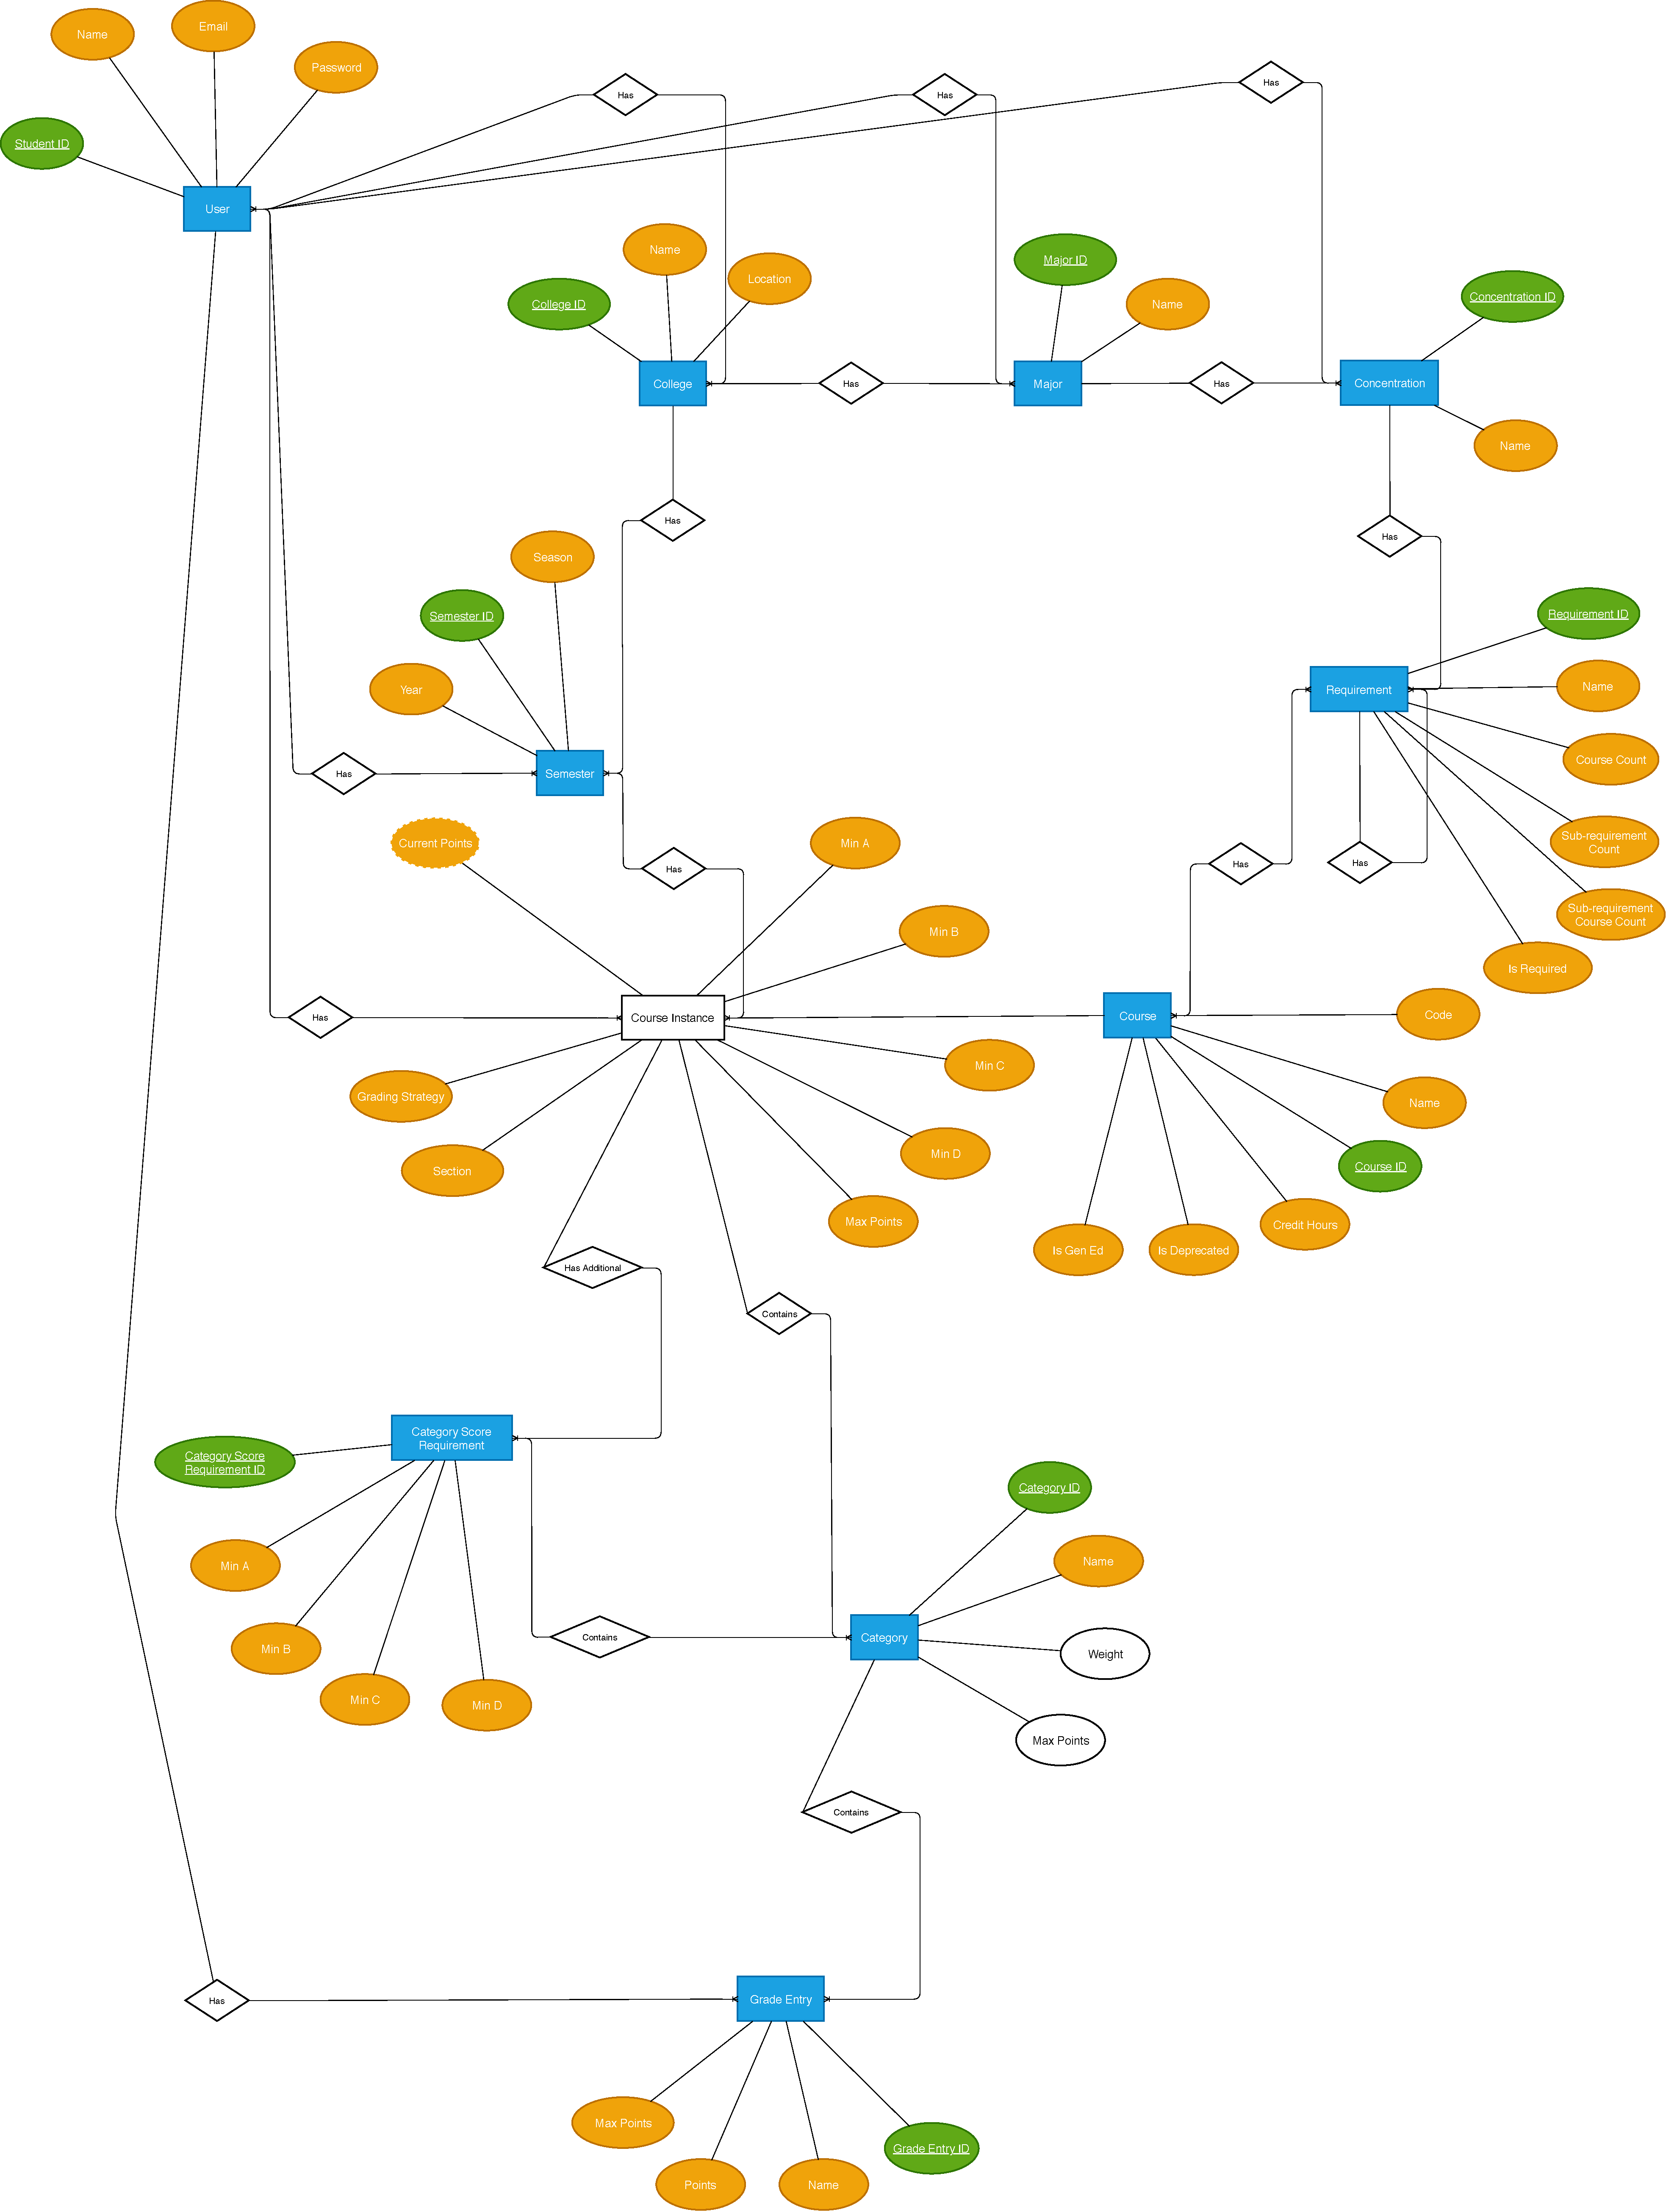
\includegraphics[width=\linewidth]{database_erd.pdf}
  \caption{Database ERD}
\end{figure}

\clearpage

\subsection{Table Schema}

\section{Conclusion}

\section{Dictionary}
\begin{itemize}
    \item \textbf{Semester}: A single semester of education consisting of courses. Each semester can
    be associated with a different educational institution; consistency is not required.
    \item \textbf{Course}: Any educational course/class occurring within a particular semester.
    \item \textbf{Section}: An equally weighted or logically grouped collection of material within a
    particular course (e.g. Homework, Tests, etc.).
    \item \textbf{Grade Entry}: A graded piece of material associated with a particular section 
    (e.g. Homework 2, Exam 1, etc.).
\end{itemize}

\end{document}
